\chapter{The High Luminosity Large Hadron Collider}
% \label{chap:HL-HLC}
% \section{An overview of the Large Hadron Collider}

% exposition on 
% the general principle of the LHC
% key parameter : luminosity, how it translates to physics, 
% how to control the luminosity, current luminosity of the LHC, how much data it has derivered
% introduce the HL-LHC

At the time of writing this thesis in 2025, the LHC has been in operation for over 13 years and delivered to each of its general-purpose detectors--ATLAS and CMS--approximately $350\,\ifb$ of proton--proton collision data at a peak center-of-mass energy of $\sqrt{s}=13$ TeV. 
Table \ref{tab:lhc-int-lumi} illustrates  the energy and quantity of data collected over the LHC runs. 
An instantaneous luminosity of $2\times 10^{34} \, \mathrm{cm}^{-1}s^{-1}$ was achieved in 2018 and has been maintained until now, furnishing an integrated luminosity of $350\,\mathrm{fb}^{-1}$, well above the initial goal of $300\,\mathrm{fb}^{-1}$.

\begin{table}[h!]
    \centering
    \begin{tabular}{|c|c|c|}
    \hline
        Run & Period & Integrated luminosity $[\ifb]$ \\ \hline
        1 & 2010 -- 2012 & 29.2 \\
        2 & 2015 -- 2018 & 159.8 \\
        3 & 2022 -- 2025 & 160.4 \\ \hline \hline
        \multicolumn{2}{|c|}{Total} & 349.4 \\
        \hline
    \end{tabular}
    \caption{The integrated luminosity delivered to the ATLAS detector by the LHC as of September 2, 2024. }
    \label{tab:lhc-int-lumi}
\end{table}

Even before the nominal LHC operation, the High-Luminosity LHC (HL-LHC) project was established to fully exploit the collider's discovery potential. 
The aim is to increase the instantaneous luminosity to $5\times 10^{34} \, \mathrm{cm}^{-1}s^{-1}$, reaching up to $7.5\times 10^{34} \, \mathrm{cm}^{-1}s^{-1}$, 3.75 times higher than the current rate. 
As such, the total integrated luminosity at the end of the HL-LHC will attain $3000\,\mathrm{fb}^{-1}$, 10 times the data planned for the baseline LHC.
Increasing luminosity proportionately increases the rate of event production $\expval{N}$, since
\beq
\label{eq:hllhc:1}
\expval{N_{pp\to X}}=\mathcal{L}\sigma_{pp\to X}
\eeq
where $\mathcal{L}$ and $\sigma_{pp\to X}$ are respectively the instantaneous luminosity and the production cross-section of the final state $X$. 
For example, the production cross-section of a Higgs boson is $\sigma_{pp\to H}=50 \, \mathrm{pb}$, so the average Higgs production rate at the current luminosity $\mathcal{L} = 2\times 10^{34}\, \mathrm{cm}^{-1}s^{-1}$ is 
\beq
\label{eq:hllhc:2}
\expval{N_{pp\to H}}= [2\times 10^{34}\, \mathrm{cm}^{-1}s^{-1}] \times [50 \times 10^{-36}\, \mathrm{cm}^{-2}] = 1\, \mathrm{Hz},
\eeq
i.e. one Higgs boson produced every second.

\begin{figure}[h!]
    \centering
    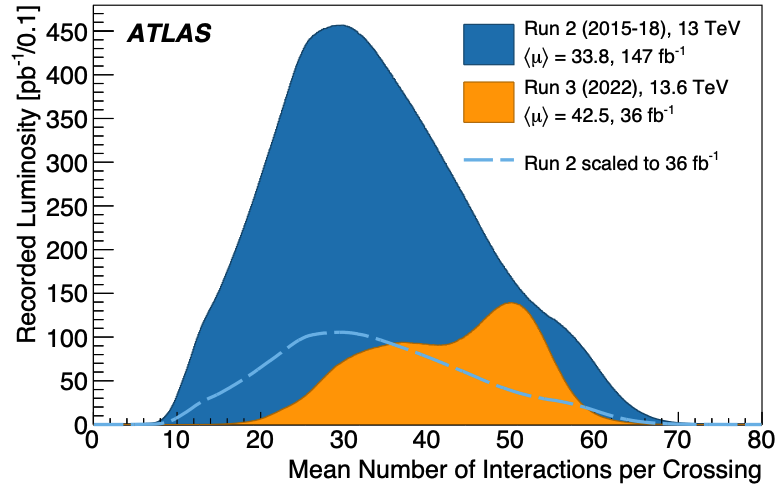
\includegraphics[width=0.65\linewidth]{figures/pileup-dist.png}
    \caption{Distribution of pile-up multiplicity $({\mu})$ in proton--proton collision at the ATLAS interaction point during Run 2 and the data taking period in 2022 of Run 3. The dashed line represents a rescaled Run 2 distribution such that its integral is the same as that of the Run 3 distribution. $\expval{\mu}$ denotes the distribution mean. Figure taken from reference~\cite{software-perf-atlas-run3}.}
    \label{fig:pileup-dist}
\end{figure}

All interactions that can occur in $pp$ collision are boosted by higher luminosity. 
The rate not only of interesting collision events, but also of soft background events increases.
The gross number of proton--proton interactions per bunch crossing, called the \textbf{pile-up multiplicity} and denoted $\mu$, can be estimated using equation \eqref{eq:hllhc:1} by noting that the total $pp$ cross-section is of order $100\,\mathrm{mb}$.
Figure \ref{fig:pileup-dist} shows the distribution of the average pile-up at the ATLAS interaction point during Run 2 and the first year of Run 3.
While pile-up primarily ranged from 20-40 in Run 2, it peaks around $\mu=50$ in a large fraction of events recorded by ATLAS in Run 3.
The HL-LHC is designed to achieve a peak luminosity of $7.5\times 10^{34} \, \mathrm{cm}^{-1}s^{-1} $, corresponding to and average pile-up of $\expval{\mu}=200$.

To prepare for this major change in operating conditions, the accelerator as well as all experiments at the LHC will undergo significant upgrades during the Long Shutdown after Run 3, between 2026 and 2029. 
In the ATLAS Collaboration, both hardware and software upgrades will take place, among which the most relevant to this thesis is the replacement of the current Inner Detector described in section \ref{subsect:inner-detector} by a new all-silicon \textbf{Inner Tracker}, commonly known as the \textbf{ITk}. 
Chapter \ref{chap:itk} describes the design and simulation of the ITk, and chapter \ref{chap:atlas-reco-chain} the current track reconstruction chain, concluding with the challenges associated with this process at high pile-up. 
This difficulty motivates the development of a novel, accelerated tracking algorithm, which constitutes the rest of this thesis.

% \section{The ATLAS Inner Tracker}



% \section{The ATLAS Inner Tracker}

% \section{A roadmap to ATLAS LH-HLC}